\section{Energy-based Tree Reconfiguration}
\label{OptimalTree}

RPL uses ETX which is the expected number of transmissions to reflect the link reliability and the expected latency on the channel. The ETX value is calculated by the node in selecting the next hop route. In order to find the optimal tree, it is assumed that RPL has selected the best routes and MCRP further improved the selected paths by switching to better channels for the transmissions. However, the current best paths do not take into account the nodes residual energy. This could drain the battery of certain nodes quicker than other nodes. RPL can reconstruct the tree as the result of MCRP. The routes might have better reliability in the new channel than it was previously.

%/////Explanation of ETX - The distance from the node relative to the other nodes with respect to the root is called rank. The rank increases away from the root and decreases when it is nearer to the root. Rank is used to avoid routing loop in the topology as the node’s position relative to the other nodes is known.////kind of like Dijkstra

\subsection{Details of Optimal Tree Reconfiguration}

In order to maximise the network lifetime, MCRP has to consider swapping the paths. The optimal tree swapping has to take into account the number of children and descendants to balance the energy consumption in the network based on the residual energy of the nodes. 
The proposal aims to find the tree that could maximise the node with the minimum lifetime. There are three possible solutions that are considered; (a) swap the parent of node $i$, (b) swap the children of node $i$, and (c) swap the descendants of node $i$ that are not the children. However, swapping the parent of the minimum lifetime node does not improve the node lifetime as the number of children and descendants remain same. Thus, only option (b) and (c) are further investigated.  

\begin{equation}
l_i = \frac{e_i}{{(d_i + 1)t_{ip(i)} + \sum_{j \in c(i)} (d_j + 1)t_{ji}}}
\label{optimalEq}
\end{equation}

Equation \ref{optimalEq} shows MCRP optimal tree calculation where $l_i$ is the node $i$ current lifetime based on the node's remaining energy $e_i$ (in percentage), $d_i$ is the number of descendants, $t_{ij}$ represents the number of transmissions on average from node $i$ to node $j$, $p(i)$ refers to the parent of $i$ and $c(i)$ is node $i$ set of children.

\begin{algorithm}
\caption{Pseudo-code for MCRP optimal tree algorithm}
\label{mcrp_algo}
\begin{algorithmic}[]
\\\textbf{Notations}
%\\$e_i$ is the node battery power
\\$l_i$ is the node lifetime
\\$c_i$ is the number of node $i$ children
\\$d_i$ is the number of node $i$ descendants
%\\$t_{ij}$ is the number of transmissions on average from $i$ to $j$
%\\$p(i)$ is the parent of node $i$
%\\$c(i)$ is the set of node $i$ children
\\\textbf{Pseudo-code}
\\Form tree based on MCRP
\\Update battery level for all nodes
\\Update all nodes $l_i$, $c_i$, $d_i$
\\minimum $\leftarrow$ 0
\\previousSwapNode $\leftarrow$ 0 
  \While{node $\neq$ previousSwapNode}
    \State Find node with minimum $l_i$
    \State List all potential $c_i$ and $d_i$ swap
	\If{$c_i$ and $d_i$ swap $l_i$ $>$ minimum} %to avoid cycle
		\State Recalculate all nodes $l_i$
		\If{all new nodes $l_i$ $>$ minimum}
			\State Update tree
			\State New tree is optimal
		\Else
			\State Revert to previous optimal tree
		\EndIf
			\State previousSwapNode $\leftarrow$ node
	\Else
		\State Current tree is optimal
	\EndIf
  \EndWhile
\end{algorithmic}
\end{algorithm}

Algorithm \ref{mcrp_algo} describes the swapping processes based on the nodes lifetime calculated from Equation \ref{optimalEq}. It considers all available paths between the nodes and shows all potential topologies before deciding on the optimal tree.
It is assumed that all nodes residual energy and the paths are known. Both the nodes battery and the link conditions can deteriorate over time. However, it is assumed that the current selected paths are the favourable routes selected by the MCRP, thus, only the battery level of the nodes is the variable. The topology is changed accordingly where the nodes that have the minimum value is selected to balance the network in term of the battery, link conditions and the number of children and descendants. The network is considered as balanced in term of the lifetime which means, the number of nodes and descendants connected might not be fairly distributed as the battery level vary in each node.

\subsection{Illustrative Example}

Figure \ref{fig:ot} is an illustrative example to explain the algorithm proposed. Assumed that the tree formed in Figure \ref{fig:ot-1} is the current optimal tree after running MCRP processes. Each node is labelled with the battery level, represented in percentage for simplicity. It can also be represented in volts or Joules. The lines between the nodes represent routes in different channels where dotted lines are the potential routes and the solid lines are the current routes. The values represent the link conditions in terms of the number of successful expected transmission between the two nodes. The values of the links are the expected transmission taken only for the upwards route as the links downwards could have different values due to the different transmission and reception channels on each node thus different link quality. 
%The main reason for this difference is due to the two hops algorithm implemented in MCRP. 
The transmission and reception channels of a node cannot be the same to avoid interference with nearby nodes.
%Figure \ref{fig:graphTree1-2} is the simplified graph of Figure \ref{fig:graphTree1} where the nodes are (labelled?) with their lifetime calculated based on the paths (solid lines) and the potential edges are the link condition values of the node pair.

The figure shows that node 2 has the most descendants which consequently reduce the node lifetime as it has to forward more packets than any other nodes. Initially, the topology is formed based on the least value on the paths. In order to optimise the tree, the overall network lifetime is considered where paths that are not the minimum could be chosen as the route as it prolongs the overall functionality of the network. In this example, node 2 has the minimum lifetime. It can be maximised through swaps. 

There are several potential swaps to improve node 2 lifetime that includes both the children which are node 5 and 6, and the children of children, node 7 and 8. Figure \ref{fig:ot-2} shows node 5 swaps to node 4 instead of its initial node 2 and the network lifetime is calculated. Node 2 lifetime is improved, however, node 1 has a lower lifetime than the initial minimum value as the result of swapping. Node 1 now has 5 descendants while node 2 only has one when it initially had 4. In order to reduce the number of unnecessary swap, once the maximum minimum lifetime is found, all nodes lifetime values are checked to ensure that they have higher lifetime than the initial minimum lifetime regardless of the maximising the minimum node to avoid endless cycle of swaps. While the swap done by node 5 improves node 2 lifetime, node 1 lifetime deteriorates to a value lower than the minimum. The network reverts to the previous topology that is better than the new swap. Node 5 tries and swaps to node 6, then node 6 swaps to node 8. However, the potential topology is not improved. Node 2 then swaps its descendants node 7 and 8.

When node 7 is swaps to node 4 instead of node 5, the tree is improved. It can be seen in Figure \ref{fig:ot-3} that the tree is more balanced and node 2 lifetime is prolonged. As the result of swapping, node 4 lifetime is reduced as the path from node 7 to node 4 is not the smallest path value. The tree is updated as the current optimal tree. It is not yet the final optimal tree because node 8, which is another node 2 descendant has not been checked. If node 8 swap does not improve the tree, the swap from node 7 is chosen as the final optimal tree. 
Another potential swap is shown in Figure \ref{fig:ot-4} where node 8 is connected to node 6 instead of node 5. In both cases, node 2 lifetime is maximised and all nodes lifetime are above the minimum value. The tree in Figure \ref{fig:ot-3} is selected as the final optimal tree in maximising node 2 lifetime. Further investigations are required in order to decide the criteria on an optimal tree when there are several good topologies to be selected. 

Node 1 is then selected as the minimum lifetime as node 2 cannot be selected again to avoid unnecessary repetition. Optimal tree from the potential swaps for node 1 is not found thus the tree is said to be optimal. In the algorithm, the same node cannot swap again right after its previous swap. This is done to avoid oscillation which would produce similar result. The node however, could swaps in the next round as the other node swap would have changed the topology.

The swaps are assumed to happen once until the network stops functioning, thus the overheads are negligible. The swapping calculations and decisions are made by the LPBR due to sensors limitations and constraints. LPBR informs the specific nodes of the final swapping if it needs to take place. In term of energy cost, the cost is negligible as the swaps are infrequent and being controlled by the LPBR.

\begin{figure}
\centering
\subfigure[Initial tree]{\label{fig:ot-1}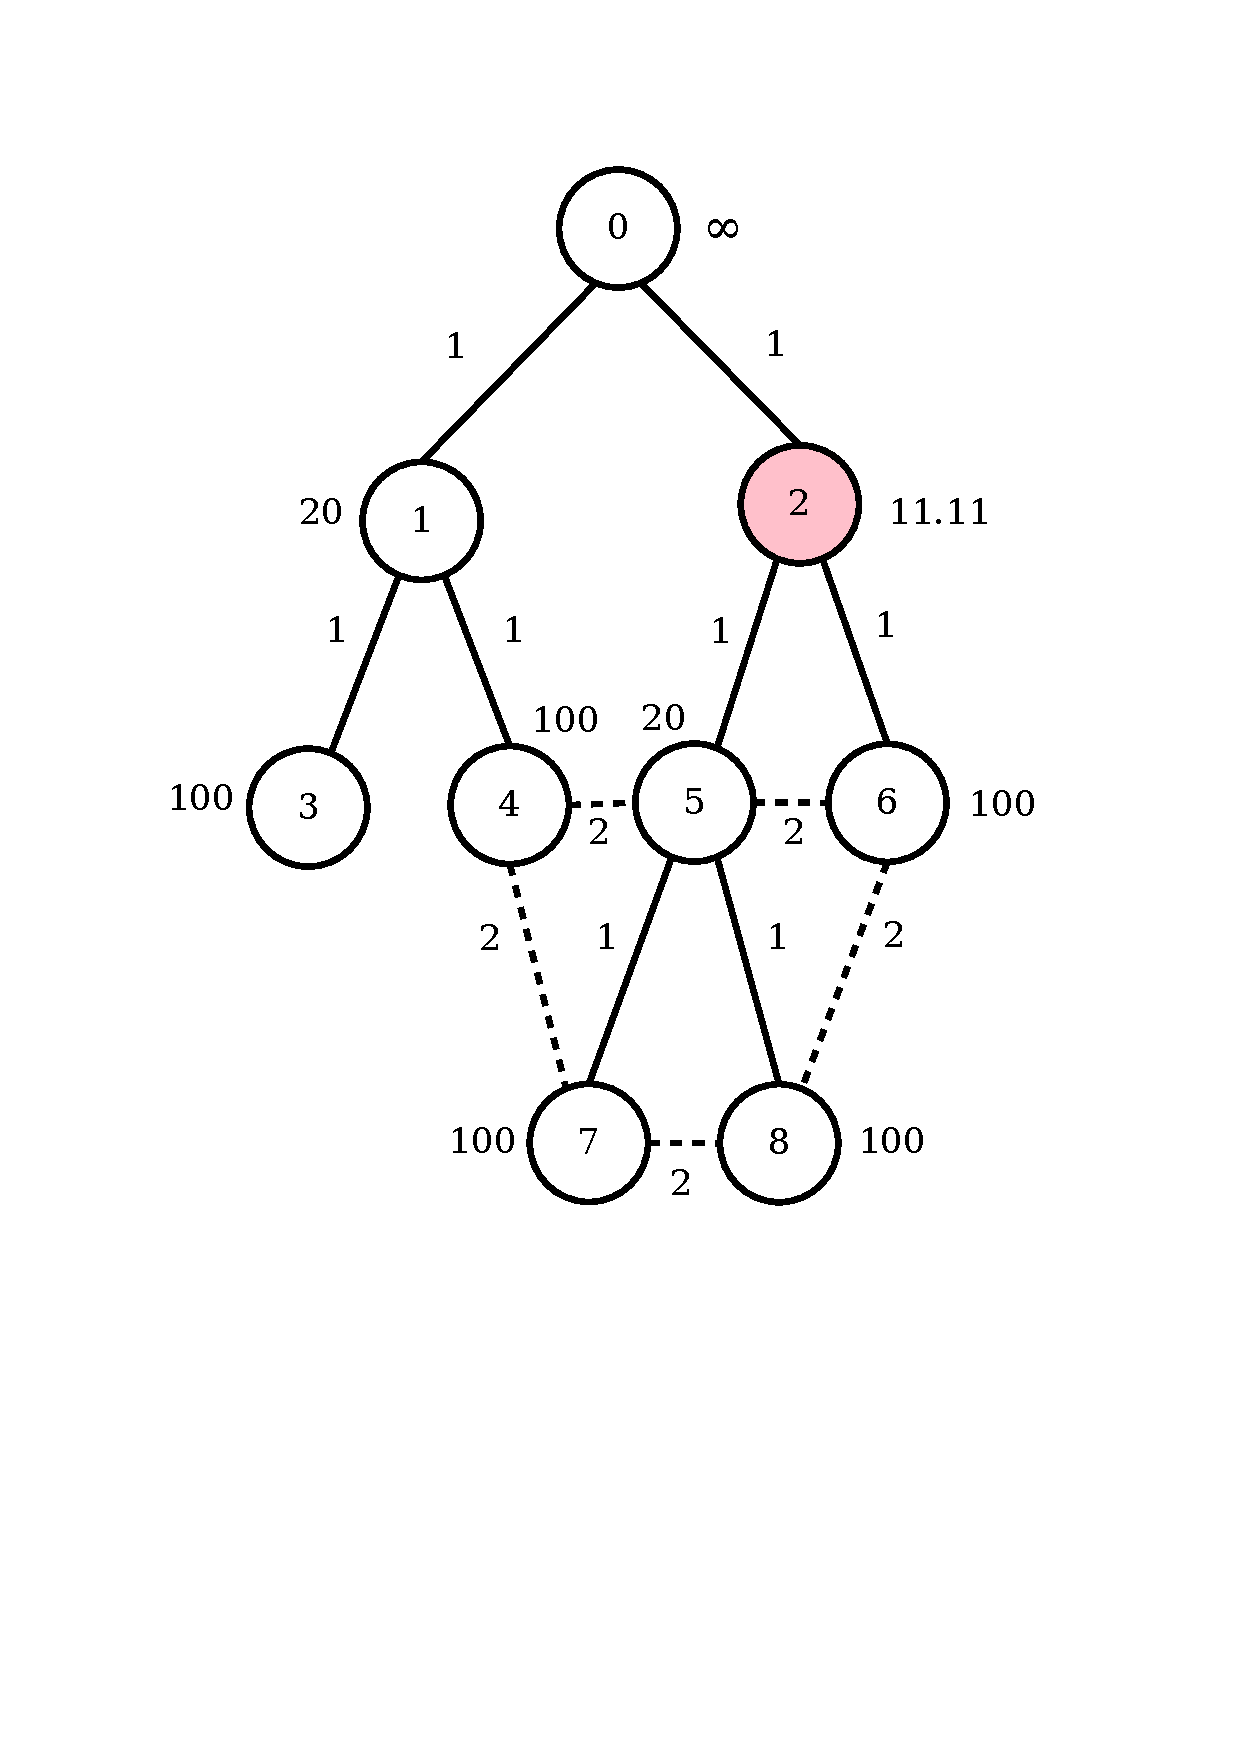
\includegraphics[page=1, trim=2cm 9cm 2cm 2cm, clip=true, totalheight=0.19\textheight]
{figures/ot1.pdf}}        
%\hfill        
\subfigure[Node 5 swaps to node 4]{\label{fig:ot-2}\includegraphics[page=2, trim=2cm 9cm 2cm 2cm, clip=true, totalheight=0.19\textheight]
{figures/ot1.pdf}}
%\hfill        
\subfigure[Node 7 swaps to node 4]{\label{fig:ot-3}\includegraphics[page=3, trim=2cm 9cm 2cm 2cm, clip=true, totalheight=0.19\textheight]
{figures/ot1.pdf}}
%\hfill        
\subfigure[Node 8 swaps to node 6]{\label{fig:ot-4}\includegraphics[page=4, trim=2cm 9cm 2cm 2cm, clip=true, totalheight=0.19\textheight]
{figures/ot1.pdf}}
\caption{Graph of the bidirectional paths in a WSN}
\label{fig:ot}
\end{figure}